%% Font size %%
\documentclass[11pt]{article}

%% Load the custom package
\usepackage{Mathdoc}

%% Numéro de séquence %% Titre de la séquence %%
\renewcommand{\centerhead}{Chap. 2 : Activité introductive}

%% Spacing commands %%
\renewcommand{\baselinestretch}{1}
\setlength{\parindent}{0pt}

\begin{document}

\begin{exercice}[0][Une origine Physique.]
La notion de nombre dérivé ne s’est pas construite en jour. \\
Tout commence avec une histoire de vitesse instantanée et de chute des corps.\\
Dès l’antiquité, Galilée démontre que si on lâche d’une hauteur suffisamment grande une pierre, et si on néglige les forces de frottement qu’elle subit, cette dernière aura une cote $z(t)$ qui peut se mettre sous la forme :\\
$$z(t)=5t^2$$

\begin{center}
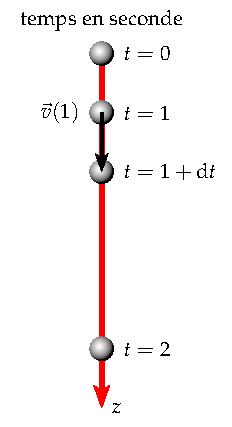
\includegraphics[scale=1]{.data/chute.pdf}
\end{center}
Remarquez ici que pour simplifier les calculs, l’axe des cotes est orienté vers le bas.
\begin{enumerate}
\item Quelle distance a parcouru la pierre au bout de 10s ?
\item Quelle est alors la vitesse moyenne pendant ces 10 premières
  secondes ?
\item Quelle distance a parcouru la pierre entre 15 et 20 secondes ?
\item Quelle est alors sa vitesse moyenne entre 15 et 20 secondes ?
\end{enumerate}
L’objectif est maintenant de trouver la vitesse INSTANTANEE à $t=1s$
\begin{enumerate}[resume]
\item Proposez une valeur approximative de cette vitesse instantanée ?
\item Proposez une méthode qui permet d’améliorer cette valeur.
\end{enumerate}
\end{exercice}

\begin{center}
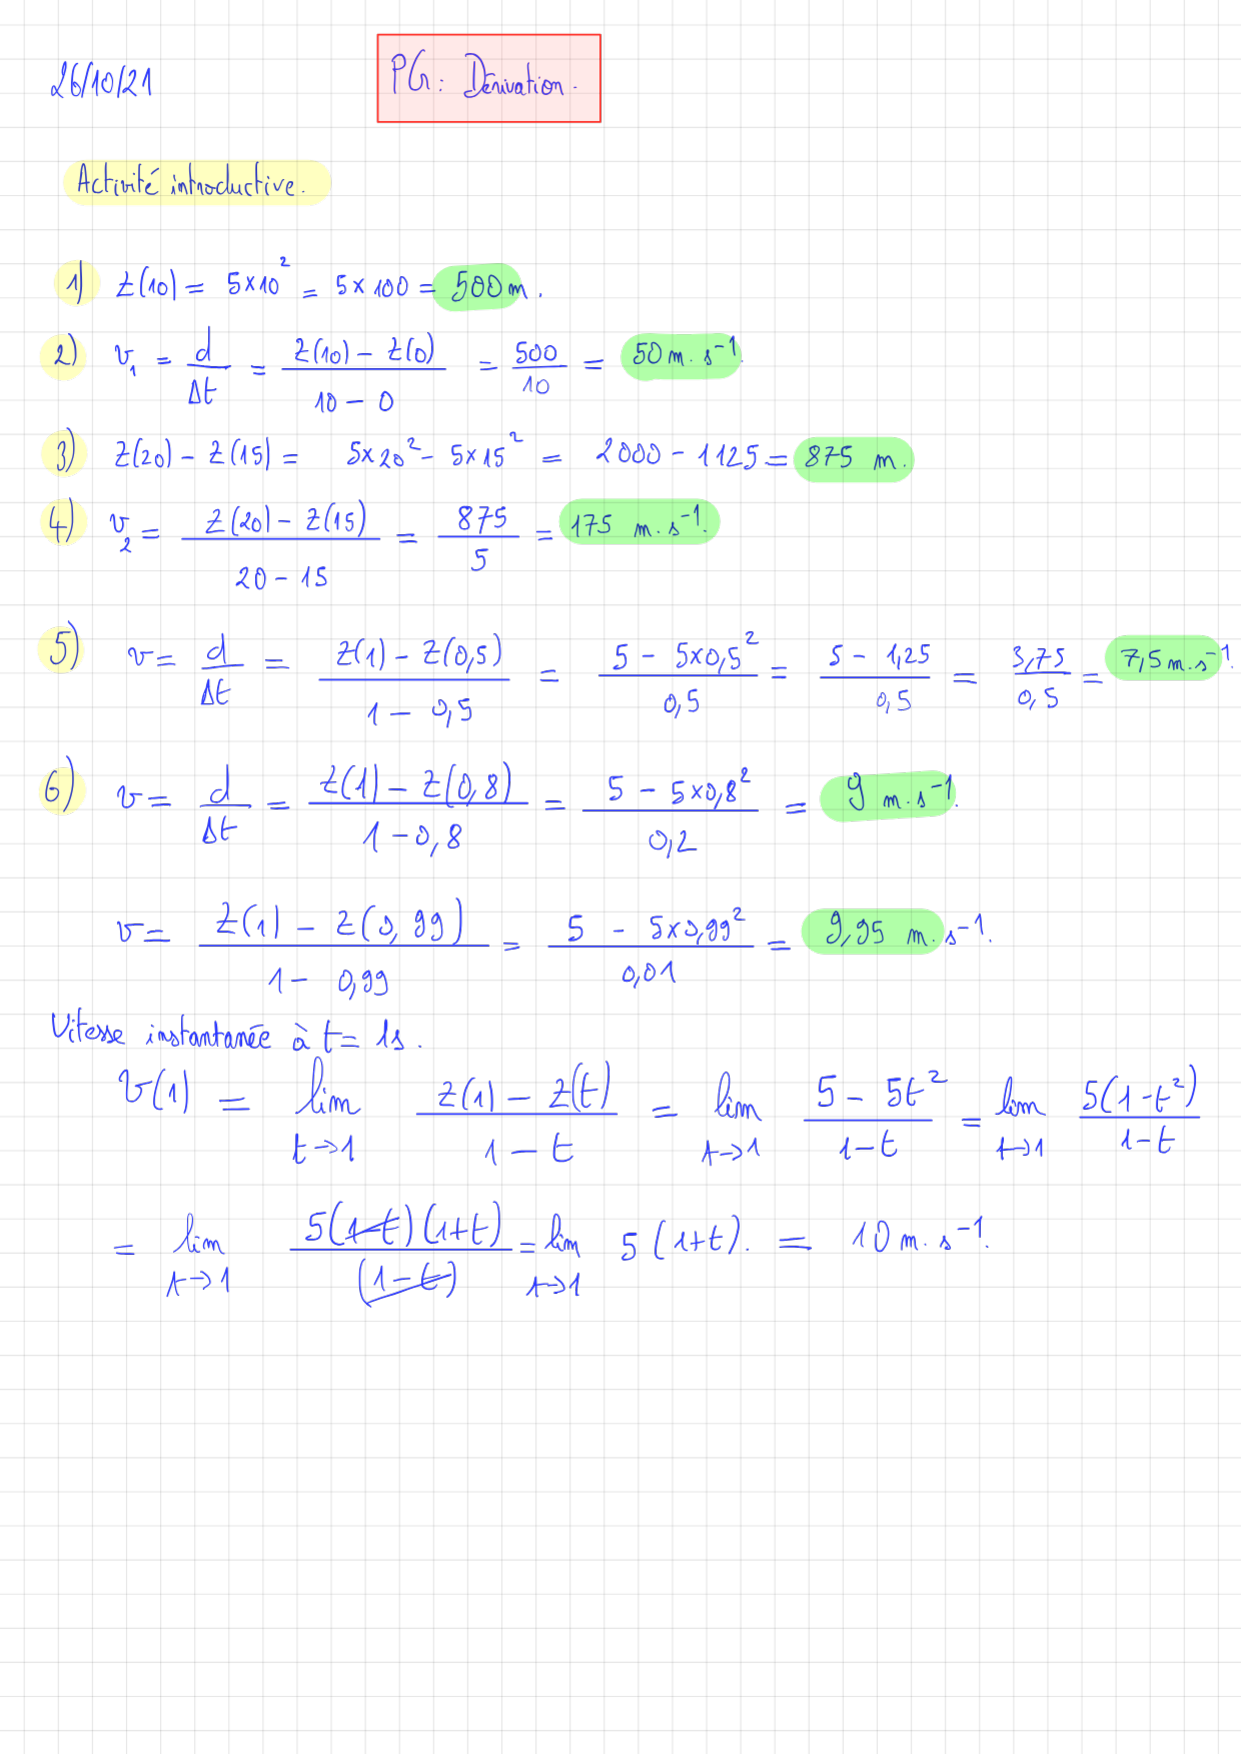
\includegraphics[scale=0.9]{.data/Derivation-corrigé.pdf}
\end{center}

\end{document}
